% !TeX root = ..\main.tex
% Chapter 2

\chapter{古诗生成与大模型}

本章主要介绍古诗生成任务的基本要求、现有技术方案以及古诗质量的度量方法,分析现有研究的不足之处,并简要介绍DeepSeek-R1与VL2两个大模型,为后续的系统设计方案作铺垫。

\section{古诗生成任务概述}

古诗生成任务要求模型能够根据需要生成符合要求的中国传统诗词,这要求模型的输出不仅能达到古诗的韵律、对仗等形式要求的建筑美,还要在内容上符合古诗的意境、情感等内涵要求。

古诗体裁多变,产生于汉朝前的古体诗形式自由、不拘泥于严格的格律,唐朝的近体诗(如律诗、绝句)与词则都格律严格。而在古诗生成任务中,往往会选择格律严格的近体诗或词作为生成目标,以便评估模型约束输出的能力。格律要求大概如下三点:

\begin{enumerate}
    \item 押韵:指诗中某些句子的末尾字使用相同或相近的韵母,形成韵脚和谐的音韵效果。律诗和绝句均要求在偶数句的句末押韵,首句可押可不押,且通常押平声韵。在唐诗中,往往要求一韵到底,即整首诗只能使用同一个韵部的字来押韵,中途不可换韵。
    \item 平仄:指汉字声调的高低,分为平声和仄声,在现代汉语中大致对应为一二声和三四声。在唐诗中,五言与七言各有不同的格律格式,如五言诗有四种基本的平仄类型,分别为“平平平仄仄”“仄仄平平仄”“仄仄仄平平”“平平仄仄平”,不同类型可在同一首诗中交替使用。此外,律诗的偶数句中的第二字须与前一句的第二字平仄相同,称为“粘连”。
    \item 对仗:指律诗中颔联(第三、四句)与颈联(第五、六句)在词性、语义、平仄等结构上形成对称关系,这也是律诗重要的特征之一。如“大漠孤烟直,长河落日圆”,前后两句的词性、语义、平仄均形成对称关系,朗朗上口。
\end{enumerate}

排律是格律的变体,其延续律诗严格的格律要求,但篇幅较长,通常在十句以上,不过押韵要求较为宽松,中途可换韵。排律的篇幅和结构更为复杂,十分考验创作者的文学功底和创作技巧,因而在传统诗歌中,排律的作品相对较少。

\section{现有方案}
……

\section{古诗质量评估}
\subsection{BLEU}
BLEU(Bilingual Evaluation Understudy),又名双语替换测评,是一种用于评估机器翻译质量的指标,核心是通过比较机器翻译结果与参考翻译之间的$n$-gram匹配情况来评估翻译质量,并以精确率(Precision)作为衡量指标。\cite{papineniBLEUMethodAutomatic2002}

具体而言,其计算候选句子中在参考句子中出现的$n$-gram的次数$Count$。
而为了避免导向无意义的$n$-gram重复,BLEU对候选句子中的$n$-gram计数进行截断(clip),使同一个$n$-gram的计数不超过参考句子中该$n$-gram的最大次数,即$Count_{clip}=\min\{Count,Max\_Ref\_Count\}$。

而在含有多个句子的长文本段落中,BLEU的处理单元依旧是其中的句子。对候选段落中的每个句子$\mathcal C$,计算其所有的$n$-gram的截断后计数$Count_{clip}$,再按句子累加在一起,整体除以同理得来的非截断计数$Count$,于是得到一个归一化的分数,以适用于不同长度的文本比较。修正后的精确率如式\eqref{eq:bleu_p}:
\begin{equation}
    p_n=\frac{\sum_{\mathcal C \in\{Candidate\}} \sum_{n\mbox{-}gram\in\mathcal C} Count_{clip}(n\mbox{-}gram)}{\sum_{\mathcal C \in\{Candidate\}} \sum_{n\mbox{-}gram\in\mathcal C} Count(n\mbox{-}gram)} \label{eq:bleu_p}
\end{equation}

为了结合不同$n$取值下$n$-gram的指标分数,对不同的$n$-gram分数进行加权几何平均,其中权重$\sum\omega_i=1$,如式\eqref{eq:bleu_arg}:
\begin{equation}
    \exp\left(\sum^N_{n=1} \omega_i\log p_n\right) \label{eq:bleu_arg}
\end{equation}

进一步,为了避免机器翻译生成过短的句子来提高匹配的精确率,引入了简洁性惩罚(Brevity Penalty, BP),对候选文本$\mathcal C$的长度$c$与参考文本$\mathcal R$的长度$r$进行比较,计算方式如式\eqref{eq:bleu_bp}。
\begin{equation}
    \mathrm{BP}=\left\{
    \begin{array}{lr}
        1, &c>r \\
        e^{1-\frac rc}, & c\leq r
    \end{array}
    \right. 
    \label{eq:bleu_bp}
\end{equation}

最终可得BLEU的完整公式如式\eqref{eq:bleu}:
\begin{equation}
    \mathrm{BLEU}=\mathrm{BP}\cdot\exp\left(\sum^N_{n=1} \omega_i\log p_n\right) \label{eq:bleu}
\end{equation}

BLEU的值范围在$[0,1]$之间,值越大表示翻译质量越高,但绝对的数值意义不大,因此不需要追求接近于$1$的分数。

在实际使用中,权重$\omega_i$通常设置为$\frac{1}{N}$,即$n$-gram的加权平均。例如,BLEU-$2$的权重设置为$\omega_1=\omega_2=0.5$。古诗中的词大多是一到两个字,因此古诗生成任务中通常使用BLEU-$1$和BLEU-$2$。

\subsection{ROUGE}
与BLEU类似,ROUGE(Recall-Oriented Understudy for Gisting Evaluation)同样通过比较候选文本与参考文本之间的重叠$n$-gram来衡量文本翻译的准确率,但又更适用于文本摘要等注重信息提取和保留的任务。\cite{linROUGEPackageAutomatic2004}

区别于BLEU适用准确率,ROUGE使用召回率(Recall)作为衡量指标,计算候选文本$\mathcal C$中重叠的$n$-gram的数量与参考文本$\mathcal R$中$n$-gram的数量之比。如式\eqref{eq:rouge_n}
\begin{equation}
    \text{ROUGE-n} = \frac{\sum_{\mathcal C \in\{Candidate\}} \sum_{n\mbox{-}gram\in\mathcal C} Count_{clip}(n\mbox{-}gram)}{\sum_{\mathcal R \in\{Reference\}} \sum_{n\mbox{-}gram\in\mathcal R} Count(n\mbox{-}gram)} \label{eq:rouge_n}
\end{equation}

此外,ROUGE也支持多种变体,如ROUGE-L基于参考文本和候选文本之间的最长公共子序列(LCS)来计算召回率,如式\eqref{eq:rouge_l}。
\begin{equation}
    \text{ROUGE-L} = \frac{\sum_{\mathcal C \in\{Candidate\}} \text{LCS}(\mathcal C,\mathcal R)}{\sum_{\mathcal R \in\{Reference\}}\text{Length}(\mathcal R)} \label{eq:rouge_l}
\end{equation}

\subsection{Distinct}
除了BLEU和ROUGE等基于参考文本对比的度量方法外,也有方法尝试独立地衡量文本自身的质量。其中一个例子是Distinct指标,其计算文本中独特的$n$-gram的数量与文本中所有$n$-gram的数量之比,以衡量文本中用词的多样性。\cite{liDiversityPromotingObjectiveFunction2016,liGeneratingClassicalChinese2018a} 

\subsection{Similarity}
为了衡量古诗中前后句子间的语义联系和一致性,也有研究尝试使用词向量,并基于余弦相似度来计算句子间的语义相似度。\cite{dengIterativePolishingFramework2020}

这一方法的核心在于利用词向量模型在预训练阶段学习到的句子间的语义关系,因而指标分数十分依赖词向量模型的质量。为此,本文采用清华大学自自然语言研究中心开源的Bert-CCPoem词向量模型\footnote{https://github.com/THUNLP-AIPoet/BERT-CCPoem},其在一个包含几乎所有中国传统诗词的数据集CCPC-v1.0上进行预训练,涵盖926024首古诗的8933162个句子,可提供高质量的古诗句子词向量。

\subsection{人工评估}

由于古诗体裁的高度的艺术性,过去的研究中往往会邀请人类评审来评估古诗的质量。评估往往会基于单独设计的分析角度进行,如“流畅性”、“艺术性”、“连贯性”等等,依赖于分析维度的先验设计。此外,人类评审的结果往往依赖于评审员自身的文化素养、个人品味与喜好,结果难有一致性。此外,招募具有高文学素养的人类评审员也是一个难题。

由此,本文认为可利用大模型的语言能力行使人类评审员的功能,设计一套严格的质量评估体系,作为提示词指导大模型,便可得到具有高解释性、高一致性的古诗质量评估结果。


\section{DeepSeek大模型}
\subsection{DeepSeek-R1}

DeepSeek-R1\cite{deepseek-aiDeepSeekR1IncentivizingReasoning2025}

\begin{figure}[ht]
    \centering
    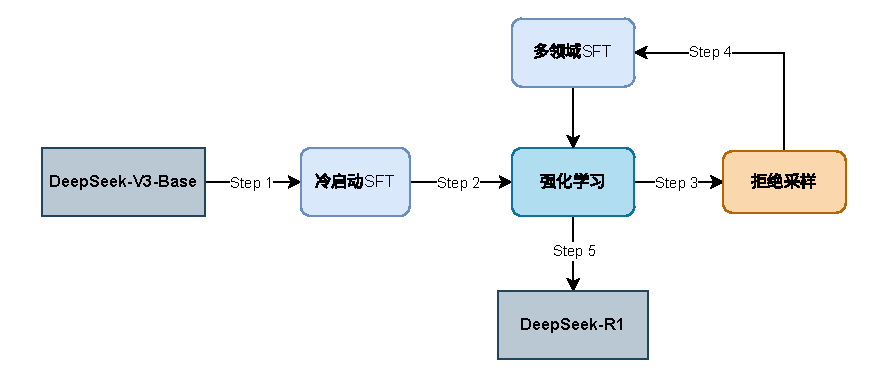
\includegraphics[width=1\textwidth]
    {figures/deepseek_r1_training.pdf}\\
    \caption{DeepSeek-R1训练过程}
    \label{fig:deepseek_r1_training} % 添加标签
\end{figure}


\subsection{DeepSeek-VL2}

DeepSeek-VL2\cite{wuDeepSeekVL2MixtureofExpertsVisionLanguage2024}采用了三阶段混合架构,包括视觉编码器、视觉-语言适配器和混合专家语言模型三大模块,如图~\ref{fig:deepseek_vl2_structure}。
\begin{figure}[ht]
    \centering
    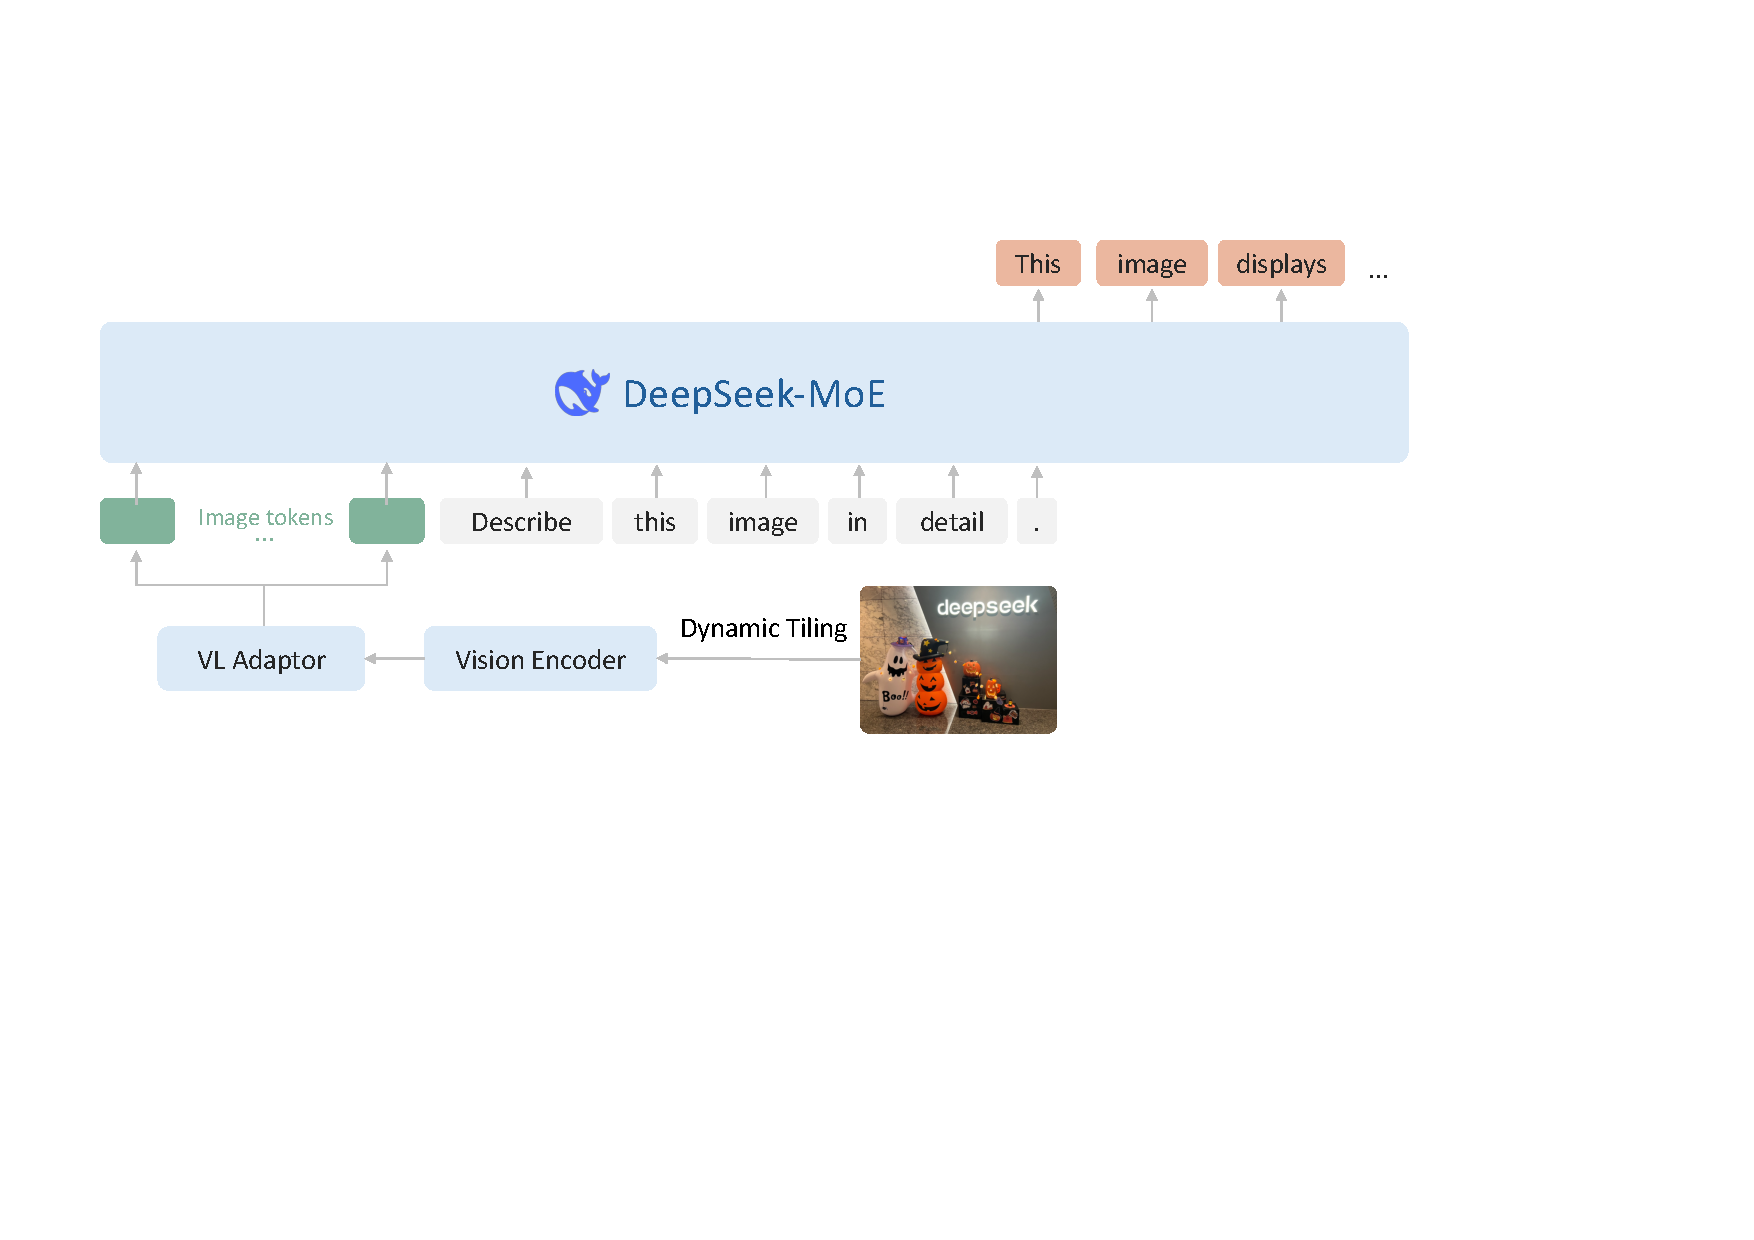
\includegraphics[width=1\textwidth]
    {figures/deepseek_vl2_structure.pdf}\\
    \caption{DeepSeek-VL2模型架构\cite{wuDeepSeekVL2MixtureofExpertsVisionLanguage2024}}
    \label{fig:deepseek_vl2_structure} % 添加标签
\end{figure}

\begin{enumerate}
    \item 视觉编码器(Vision Encoder):为了支持更大分辨率、不同比例尺寸的图像,在先前VL1模型SigLIP框架的基础上引入动态切片策略(dynamic tiling strategy),将高分辨率图像自适应分割为$384\times384$的子图块,再与全局缩略图块组合。该策略在保证宽高比不变的前提下,通过填充面积最小化算法选择最优分割方案,解决了传统固定分辨率编码导致的细节丢失问题,使模型支持最高$1152\times1152$的分辨率输入。如图~\ref{fig:deepseek_vl2_cropping_strategy}所示。
    \begin{figure}[ht]
        \centering
        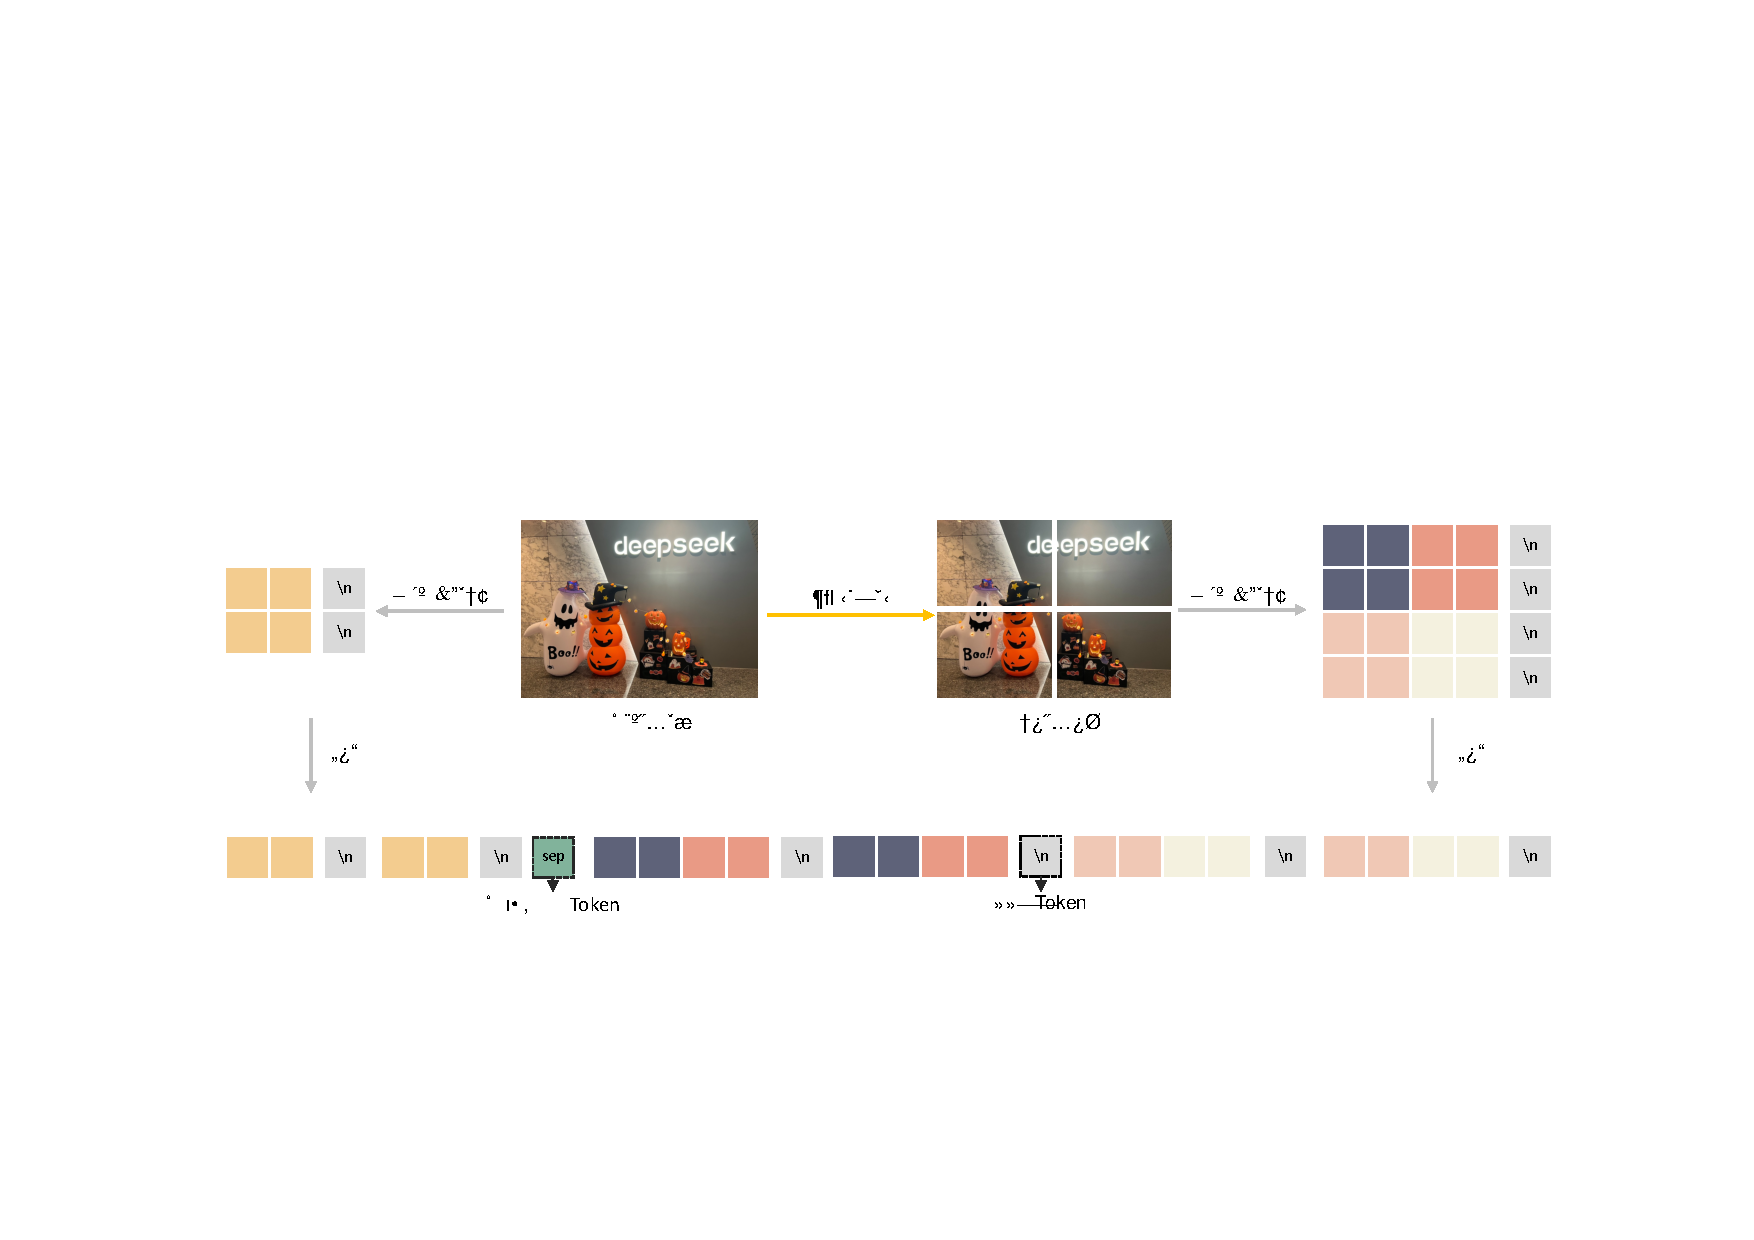
\includegraphics[width=1\textwidth]
        {figures/deepseek_vl2_cropping_strategy.pdf}\\
        \caption{DeepSeek-VL2动态切片策略\cite{wuDeepSeekVL2MixtureofExpertsVisionLanguage2024}}
        \label{fig:deepseek_vl2_cropping_strategy} % 添加标签
    \end{figure}
    \item 视觉-语言适配器(VL Adaptor):承接上一步中加入的\verb|<换行Token>|(用户区分局部图块的结束)和\verb|<视觉分隔Token>|(用于区分全局缩略图和局部图块),采用双层感知机与$2\times2$像素混洗(pixel shuffle)操作,将视觉特征维度压缩映射到文本嵌入空间。该设计在保留局部细节特征的同时,实现了跨模态特征的高效对齐。
    \item 混合专家语言模型:采用稀疏激活的专家混合架构,每个输入token动态激活Top-2专家网络。结合多头潜在注意力(Multi-head Latent Attention, MLA)机制,通过奇异值分解键值缓存压缩为潜在向量,使4096长度序列显存占用降低至传统架构的$6.7\%$
\end{enumerate}

DeepSeek-VL2的训练采用了三阶段训练范式,即先使用120万个图文对来建立跨模态关联,再使用混合$70\%$的图文数据和$30\%$纯文本数据来进行预训练,最后再专注于OCR增强和文档理解方面的监督微调。值得一提的是,DeepSeek-VL2的MoE架构包含有64个专家分组,每组都能处理特定的模态组合,并能在训练中通过负载均衡损失函数来优化专家激活分布,实现稀疏激活,从而大大提高推理效率(在总体176B的参数量下仅激活4.5B参数)。


